\subimport{archetypes/}{index.tex}
\subimport{themes/}{index.tex}
\subimport{}{futureworks.tex}
%% Define the problem + Motivation
%\begin{frame}{Scalability of Bitcoin}
%    \pgfplotsset{compat=newest}
%    \begin{figure}
%        \begin{tikzpicture}
%            \begin{axis}[
%                mbarplot,
%                xbar, xmin=0, xmax=2000,
%                width=0.9\textwidth, height=4cm, enlarge y limits=0.5,
%                xlabel={Transactions per second},
%                symbolic y coords={Visa, PayPal, Bitcoin},
%                ytick=data,
%                point meta=x, nodes near coords, nodes near coords align={horizontal},
%                ]
%                \addplot[draw=TolDarkBlue, fill=TolDarkBlue!70] coordinates {(2000,Visa) (155,PayPal) (7,Bitcoin)};
%            \end{axis}
%        \end{tikzpicture}
%    \end{figure}
%\end{frame}
%\note{
%    \begin{itemize}
%        \item Paper not directly for Bitcoin, but good example
%        \item Visa-level throughput
%        \item Another problem: Pushing number of transactions near the capacity of a block increases fees.
%        \item Also Latency in Bitcoin: potentially up to 10 minutes or even more. Visa has around 1 second.
%    \end{itemize}

%}

%\begin{frame}{Scalability of Bitcoin --- The Problems}
%    % Define the problem
%    \begin{itemize}
%        \item Bootstrapping size
%            \begin{itemize}
%                \item Hundreds of megabytes -- hundreds of gigabytes
%            \end{itemize}
%        \item Every node must process every transaction
%        \item Fixed max size for blocks (currently 1--2 mb)
%        \item Much storage necessary
%            \begin{itemize}
%                \item 2000 t/s $\times$ 0.5 kb $\sim$ 1 mb/s
%                \item 1 mb/s $\times$ 60 $\times$ 10 $=$ 600 mb per block
%            \end{itemize}
%    \end{itemize}
%\end{frame}
%\note{
%    \begin{itemize}
%        \item I.e.\ every 10 minutes, 600 mb of data is created that needs to be saved forever --- however only on a few nodes.
%        \item All points are not a problem for Bitcoin itself, but only if we want to scale it. If we want Bitcoin to sustain more than 7 tps, these points are going to be a problem
%        \item Scaling bitcoin means more centralization --- only nodes with enough resources (storage) will be able to play the game.
%    \end{itemize}
%}

%\begin{frame}{Scalability of Bitcoin --- Previous Efforts}
%    % (Briefly) discuss earlier work
%    \centering
%    %\begin{minipage}{.47\textwidth}
%    %\end{minipage}\hfill%
%    %\begin{minipage}{.40\textwidth}
%    %  \centering
%    %   \alert{Latencies} of several minutes
%    %   \alert{Slow bootstrapping}
%    %\end{minipage}
%\end{frame}
%\note{
%    \begin{itemize}
%        \item Scale-out = does it scale to thousands of nodes?
%            \begin{itemize}
%                \item ByzCoin does not scale-out experimentally to more than a few hundred nodes.
%            \end{itemize}
%        \item Elastico: First system to experimentally prove that sharding is a viable approach for an open blockchain system. However, not secure because race conditions in shards and shards are too small = high failure rates in a Byzantine setting.

%    \end{itemize}
%}

%\begin{frame}{Key Challenges}
%    A nice scalable system has to\ldots
%    \begin{itemize}
%        \item Speed up consensus
%            \begin{itemize}
%                \item \textuparrow throughput
%                \item \textdownarrow latency of transactions
%            \end{itemize}
%        \item Accommodate more data
%            \begin{itemize}
%                \item Scaling up~~~~ $\rightarrow$ ~~~ \textuparrow~transactions~~~~ $\rightarrow$ ~~~ \textuparrow~data in blockchain
%            \end{itemize}
%    \end{itemize}

%    \centering
%    \vfill
%    \pause
%    \alert{And we still want it secure and decentralized}

%    %Also, by assigning clients randomly to new shards every epoch, leads to clients needing to update more often
%    %Therefore to not bottleneck: Pruning ledger
%\end{frame}
%\note{
%    \begin{itemize}
%        \item
%    \end{itemize}
%}



%\begin{frame}{Key Contributions}
%    \centering
%    \begin{minipage}{.52\textwidth}
%    \end{minipage}\hfill%
%    \begin{minipage}{.44\textwidth}
%        ``OmniLedger is a new \alert{scalable} distributed ledger that provides \alert{secure}, \alert{decentralized}, \alert{horizontal} \alert{scaling}''
%    \end{minipage}
%\end{frame}
%\note{
%    \begin{itemize}
%        \item
%    \end{itemize}
%}

%%%%%%%%%%%%%%%%%%%%%%%%%%%%%%%%%%%%%%%%%
%\section{Key Ideas}
%%%%%%%%%%%%%%%%%%%%%%%%%%%%%%%%%%%%%%%%%

%\begin{frame}{What is OmniLedger?}
%    Techniques:
%    \begin{itemize}
%        \item New parallel consensus algorithm
%        \item Sharding
%            \begin{itemize}
%                \item Secure assignment of nodes into shards
%                \item Atomic commit to maintain cross-shard consistency
%            \end{itemize}
%        \item Compact state blocks (``checkpoints'')
%    \end{itemize}
%\end{frame}
%\note{
%    \begin{itemize}
%        \item They use the somewhat same setting as Bitcoin. Epoch-level DL, Public Key Infrastructure, Anti-sybil tokens (e.g. Proof-of-work), gossiping mechanism...
%        \item Sharding: the network nodes are split into subgroups, each of which validates a designated portion of the system's state.
%    \end{itemize}
%}

%\begin{frame}{Parallel Consensus Algorithm}
%    \centering
%\end{frame}
%\note{
%    \begin{itemize}
%        \item The idea:
%            \begin{itemize}
%                \item A strict ordering is not needed, and can be replaced by a consistent partial ordering
%                \item Instead of forcing a strict total ordering of blocks
%                \item it is better to allow clients to commit transactions in parallel.
%                \item However, we need to make sure that conflicting transactions are \emph{not} committed concurrently. Therefore we need to identify dependencies between committed transactions.
%            \end{itemize}
%        \item They do not mention how they generate the DAG and how it is maintained
%    \end{itemize}
%}



%\begin{frame}{Sharding}
%    \centering
%    How to shard?
%    \vspace{.75cm}
%    \begin{itemize}
%        \item Easy: A trusted party to divide the nodes
%            \begin{itemize}
%                \item \ldots~but that makes it centralized
%            \end{itemize}
%        \item Instead, RandHound is chosen and extended
%            %\begin{itemize}
%            %   \item \ldots~but any other publicly verifiable decentralized method could be used
%            %\end{itemize}
%    \end{itemize}
%\end{frame}
%\note{
%    \begin{itemize}
%        \item Their rationale for RandHound is that they want to keep their system separate from Bitcoin and as such have chosen RandHound since it does not rely on a blockchain-based system.
%        \item RandHound is protocol for generating fresh randomness on demand
%        \item It produces decentralized randomness
%    \end{itemize}
%}

%\begin{frame}{Sharding with (extended) RandHound}
%    \begin{itemize}
%        %\item Nodes are randomly distributed into shards
%        \item RandHound requires a ``trusted'' leader
%            \begin{itemize}
%                \item Chicken-and-egg problem
%                \item Therefore, a leader in each shard is randomly chosen by lottery
%                \item Leader abuse is detectable in the RandHound protocol
%                    \begin{itemize}
%                        \item Leader loses his right to participate in this epoch (and thus cannot gain reward)
%                        \item RandHound is restarted
%                    \end{itemize}
%            \end{itemize}
%        \item The leader uses output of RandHound to assign nodes into shards
%        \item The leader randomly selects a leader for each shard
%    \end{itemize}
%\end{frame}
%\note{
%    \begin{itemize}
%        \item Proved: 1800 hosts, an honest leader will be selected after at most 12 rounds, approx. 3 hours.
%        \item Since an epoch is a day or more, 3 hours in the worst case seems reasonable
%    \end{itemize}
%}

%\begin{frame}{Sharding and Atomic Commits}
%    \begin{itemize}
%        \item Transactions can touch more than one shard
%            \begin{itemize}
%                \item e.g.\ have several input coming from multiple shards
%            \end{itemize}
%        \item Transactions that touch several shards need to commit atomically
%            \begin{itemize}
%                \item Otherwise, there's a risk of locking funds indefinitely
%            \end{itemize}
%        \item Atomic Commits guarantee that either:
%            \begin{itemize}
%                \item[a)] A transaction is fully committed in all shards it touches
%                \item[b)] The client of the transaction holds a proof-of-rejection that enables reclaiming locked funds
%            \end{itemize}
%    \end{itemize}
%\end{frame}
%\note{
%    \begin{itemize}
%        \item
%    \end{itemize}
%}

%\begin{frame}{Sharding and Atomic Commits}
%    \begin{itemize}

%        \item Each leader of the input shards must:
%            \begin{itemize}
%                \item Validate the transaction (i.e.\ check that the inputs may be spent)
%                \item Return a \alert{proof-of-acceptance} or \alert{proof-of-rejection}
%                    %\item Lock the funds, i.e.\ make it unspendable for now
%            \end{itemize}
%        \item Afterwards, the client will publish his proof:
%            \begin{itemize}
%                \item to input shard leaders in case of rejection (to reclaim funds)
%                \item to output shard leaders to go through the with transaction
%                    \begin{itemize}
%                        \item The output shard leaders will add the transaction to the next block
%                    \end{itemize}
%            \end{itemize}
%    \end{itemize}
%\end{frame}
%\note{
%    \begin{itemize}
%        \item Rejection = the client is able to reclaim locked funds later
%    \end{itemize}
%}

%\begin{frame}{Compact State Blocks (``Checkpoints'')}
%    \centering
%\end{frame}
%\note{
%    \begin{itemize}
%        \item The idea:
%            \begin{itemize}
%                \item At the end of each epoch, the leader of a shard creates the state block
%                \item All nodes in the shard verify that it is correct.
%                \item All nodes drop all smaller blocks and only store the state block
%                \item = Proving transaction is valid is faster
%                \item = Bootstrapping is more efficient (two orders of a magnitude)
%                \item Also since nodes shift shard periodically, they need to redownload --- but only the last state block in that shard.
%            \end{itemize}
%    \end{itemize}
%}

%\begin{comment}
%    \begin{frame}{The Life of an Epoch}
%        \begin{enumerate}
%            \item An epoch is measured in coarse-grained units (e.g.\ days or weeks)
%            \item
%            \item
%        \end{enumerate}
%    \end{frame}
%    \note{
%        \begin{itemize}
%            \item
%        \end{itemize}
%    }
%\end{comment}

%\begin{comment}
%    \begin{frame}{???}
%        \begin{enumerate}
%            \item There are multiple blockchains alive at a given time --- one in each shard
%            \item
%            \item
%        \end{enumerate}
%    \end{frame}
%    \note{
%        \begin{itemize}
%            \item
%        \end{itemize}
%    }
%\end{comment}

%\begin{frame}{Evaluation}
%    \begin{itemize}
%        \item Experimental evaluation
%        \item Simulation of network using 60 physical machines
%            \begin{itemize}
%                \item Up to 1800 simulated hosts
%                \item Imposing latency of 100 ms per link
%                \item Limiting bandwidth to 20 Mbps
%                \item Data: Actual transactions from the first 10,000 blocks of Bitcoin's blockchain
%            \end{itemize}
%    \end{itemize}
%\end{frame}
%\note{
%    \begin{itemize}
%        \item
%    \end{itemize}
%}

%\begin{frame}{Evaluation --- Throughput}
%    \centering
%    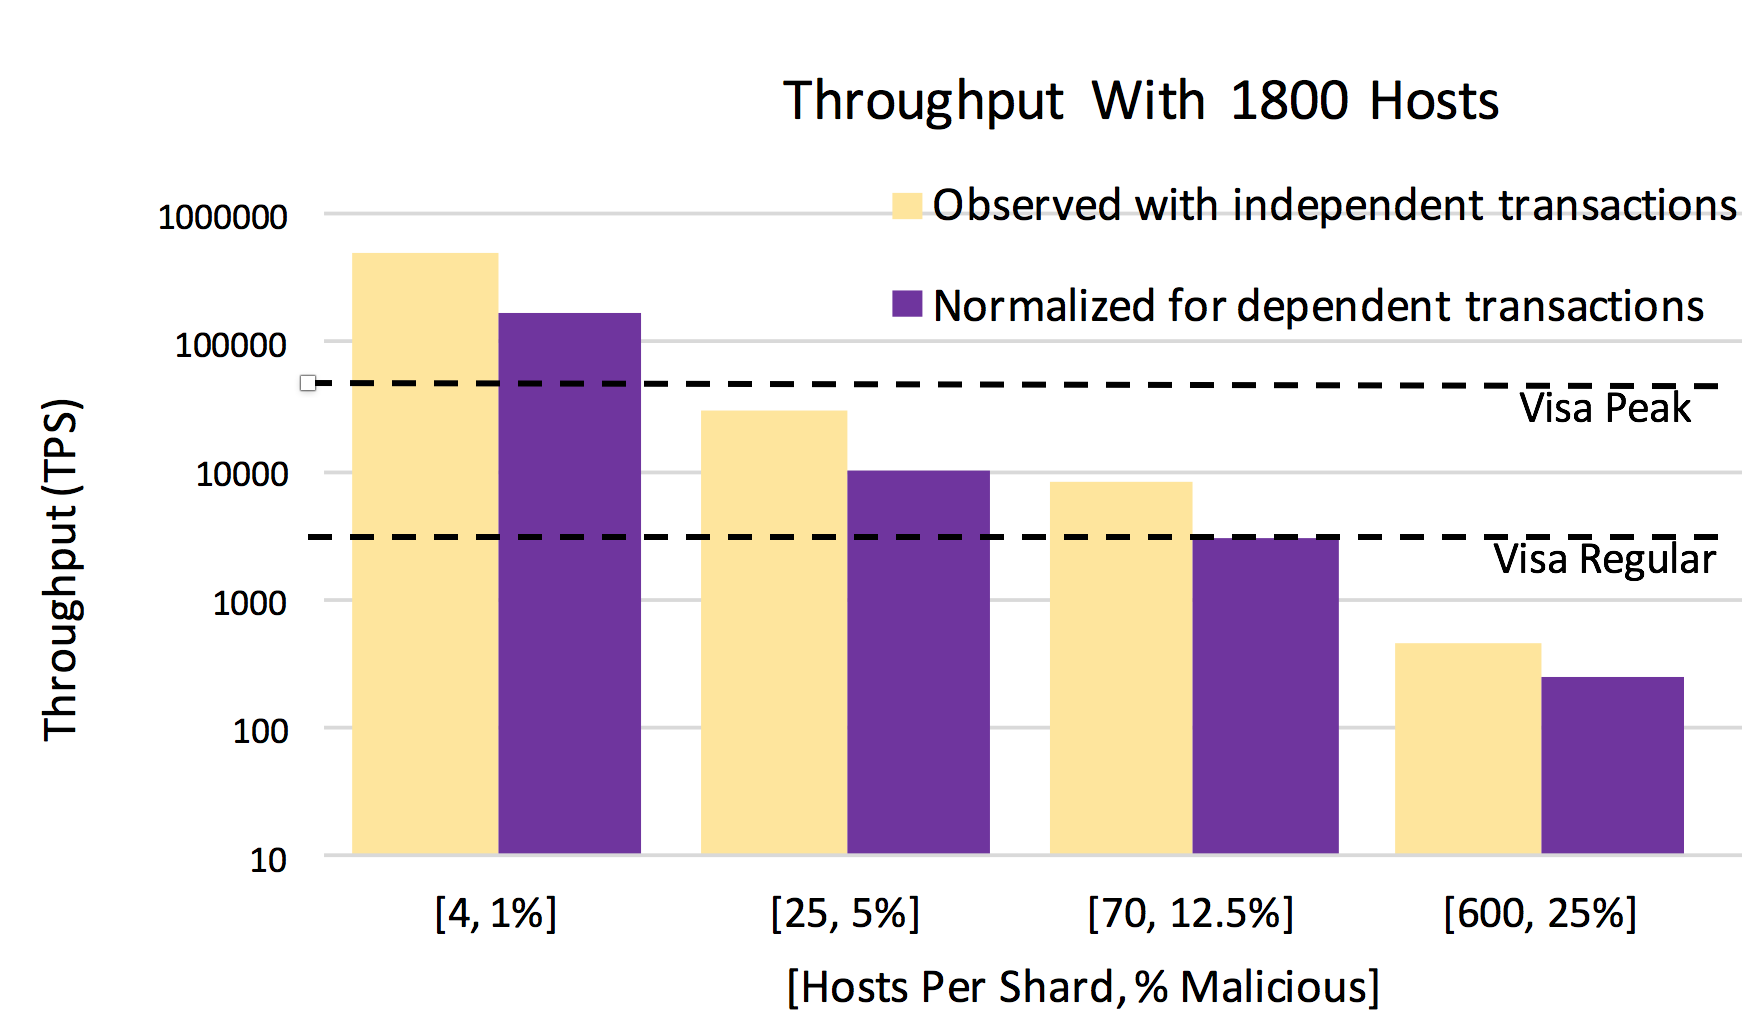
\includegraphics[height=.75\textheight]{figures/results-throughput.png}
%\end{frame}
%\note{
%    \begin{itemize}
%        \item Tunable performance based on the assumed strength of adversaries
%        \item 4 hosts = able to withstand 1 \% malicious nodes
%        \item 25 hosts = able to withstand 5 \% malicious nodes
%        \item 70 hosts = able to withstand 12.5 \% malicious nodes
%        \item 600 hosts = able to withstand 25 \% malicious nodes

%    \end{itemize}
%}

%\begin{frame}{Evaluation --- Throughput}
%    \centering
%\end{frame}
%\note{
%    \begin{itemize}
%        \item In figure, 12.5\% of nodes are malicious
%    \end{itemize}
%}

%\begin{frame}{Evaluation --- Latency}
%    \centering
%\end{frame}
%\note{
%    \begin{itemize}
%        \item In case of malicious users, ByzCoin switches to another consensus strategy, which does not scale after a few hundreds nodes.
%        \item In a system like Bitcoin, we have to assume malicious users.
%    \end{itemize}
%}

%\begin{frame}{Evaluation --- Bootstrapping Bandwidth}
%    \centering
%\end{frame}
%\note{
%    \begin{itemize}
%        \item A validator that is one month out-of-date only needs to download 40 \%, compared to Bitcoin. How this number? It isn't mentioned in the paper, just in abstract.
%        \item A new validator only needs to download 7 \% compared to Bitcoin
%        \item Makes it fast for validators to switch shard and verify any transaction
%    \end{itemize}
%}

%\begin{frame}{Evaluation --- Bootstrapping Latency}
%    \centering
%    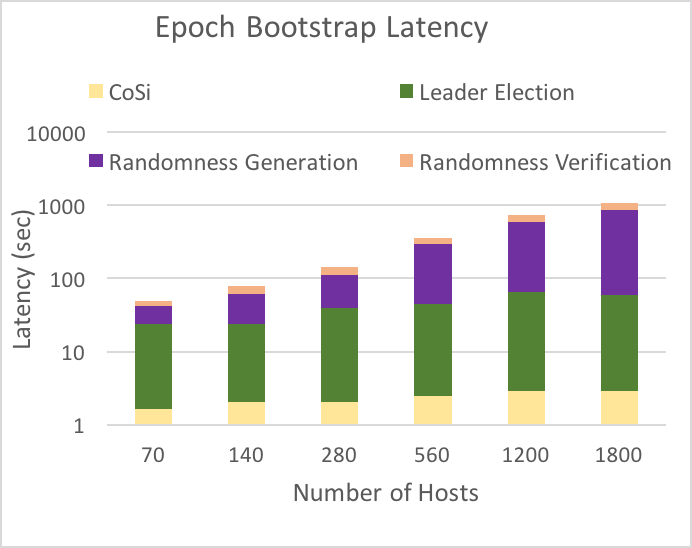
\includegraphics[height=.75\textheight]{figures/results-bootstrap-latency.png}
%\end{frame}
%\note{
%    \begin{itemize}
%        \item
%    \end{itemize}
%}

%\begin{frame}{Limitations}
%    As mentioned by paper itself:
%    \begin{itemize}
%        \item Epoch bootstrapping is still slow due to RandHound leader election
%            \begin{itemize}
%                \item However, it can be done in the background in the end of previous epoch
%            \end{itemize}
%        \item Complex transactions touching all shards are slow
%            \begin{itemize}
%                \item In this case the system is better off with one shard
%                \item Future work: Explore sharding based on locality and not just randomness
%            \end{itemize}
%    \end{itemize}

%    As mentioned by another paper:
%    \begin{itemize}
%        \item Does not work on smart contracts
%    \end{itemize}
%\end{frame}
%\note{
%    \begin{itemize}
%        \item No smart contracts because it is made with cryptocurrencies in mind.
%    \end{itemize}
%}

%\begin{comment}
%    \begin{frame}{Limitations}
%        My findings:
%        \begin{itemize}

%            \begin{itemize}
%                \item 1 day -- a few weeks
%            \end{itemize}
%        \item
%    \end{itemize}

%    %\fxnote{Can leader of shard still abuse if he has much money at stake?}
%\end{frame}
%\note{
%    \begin{itemize}
%        \item First point: However, the client sending the transaction can validate it is there, and if it believes it is censored, it can specifically request the network to commit his transaction. If still not cooperating, the honest nodes can cause a view-change.

%    \end{itemize}

%}
%    \end{comment}

%    \begin{frame}{Personal Review}
%        \begin{minipage}[t]{.45\textwidth}
%            Pros:
%            \begin{itemize}
%                \item Impressive results
%                \item Good structure of paper
%            \end{itemize}
%        \end{minipage}
%        \hfill
%        \begin{minipage}[t]{.45\textwidth}
%            Cons:
%            \begin{itemize}
%                \item Sometimes hard to follow the details
%                \item Convoluted mix of existing solutions on many levels
%            \end{itemize}
%        \end{minipage}

%    \end{frame}
%    \note{
%        \begin{itemize}
%            \item Maybe I just don't understand enough to follow their thinking.
%            \item Many details are not clear: Is every shard part of the same epoch? How do they coordinate when the epoch starts and ends? Or do every shard have their own internal epoch? Not clear to me how assignment of nodes in shards each epoch is performed? Circular dep. in DAG?
%            \item No suggestions or heuristics to decide on length of epoch
%            \item No mention of how the dag is constructed (who and how often)
%            \item Nice to have: A discussion of other approaches to randomness than RandHound
%        \end{itemize}

%    }

%    \begin{frame}{Conclusion}
%        \centering
%        Visa-level throughput and only seconds of latency\\
%        \vspace{.75cm}
%    \end{frame}

%    \begin{frame}[standout]
%        Questions?
%    \end{frame}
%    \note{

%    }
